\documentclass[]{article}
\usepackage[left=2.54cm, right=2.54cm, top=3.17cm, bottom=3.17cm]{geometry}
\usepackage{lmodern}
\usepackage{amssymb,amsmath}
\usepackage[T1]{fontenc}
\usepackage[utf8]{inputenc}
\setlength\parskip{2ex}
\raggedright

\usepackage{graphicx}
\usepackage{float}

\begin{document}
\section{Coupled Heat and Mass Transfer}
Solving the heat and mass transfer ODEs coupled is not a trivial task due to their non-linear nature. An analytic solution for the ODEs coupled has not been found so the equations can only be solved numerically. 

The following figures use the data from Miller et al. corresponding to Figure 2 in that paper. Figures \ref{heat_mass_euler_0_01_mass_lim_mass} and \ref{heat_mass_euler_0_01_mass_lim_temp} show the results for a forward Euler method and Figures \ref{heat_mass_runge_kutta_0_01_mass_lim_mass} and \ref{heat_mass_runge_kutta_0_01_mass_lim_temp} show the results for a fourth order Runge-Kutta method. For both methods a timestep of $0.01s$ was used and the final mass was limited to $0.000000001~kg$.

Figures \ref{heat_mass_runge_kutta_deltat_mass_lim_mass} and \ref{heat_mass_runge_kutta_deltat_mass_lim_temp} shows the effect of increasing the timestep  $\Delta t$.

(Apologies the figures are .png, I've tried out .eps and the figures take a while to load. Plotting data with Tikz is something I've used for reports in the past and I'll see if this works better). 

\begin{figure}[h]
	\centering
	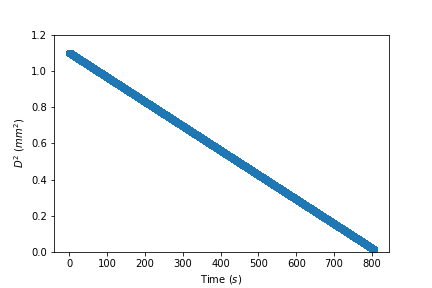
\includegraphics[width=0.8\textwidth]{heat_mass_euler_0_01_mass_lim_mass}
	\caption{$D^2$ for a droplet sized $D^2=1.1mm$ with $Re_d=0$, $T_{d_0}=282K$, $T_G=298K$, $Y_G=0$ and $\Delta t=0.01s$. Using a forward Euler method.}
	\label{heat_mass_euler_0_01_mass_lim_mass}
\end{figure}

\begin{figure}[h]
	\centering
	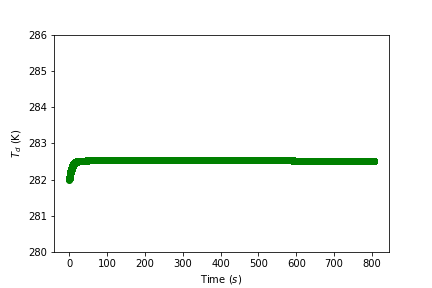
\includegraphics[width=0.8\textwidth]{heat_mass_euler_0_01_mass_lim_temp}
	\caption{$T_d$ for a droplet sized $D^2=1.1mm$ with $Re_d=0$, $T_{d_0}=282K$, $T_G=298K$, $Y_G=0$ and $\Delta t=0.01s$. Using a forward Euler method.}
	\label{heat_mass_euler_0_01_mass_lim_temp}
\end{figure}

\begin{figure}[h]
	\centering
	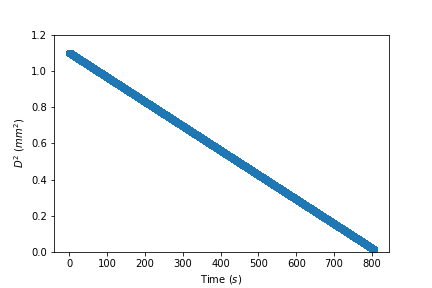
\includegraphics[width=0.8\textwidth]{heat_mass_runge_kutta_0_01_mass_lim_mass}
	\caption{$D^2$ for a droplet sized $D^2=1.1mm$ with $Re_d=0$, $T_{d_0}=282K$, $T_G=298K$, $Y_G=0$ and $\Delta t=0.01s$. Using a Runge-Kutta method.}
	\label{heat_mass_runge_kutta_0_01_mass_lim_mass}
\end{figure}

\begin{figure}[h]
	\centering
	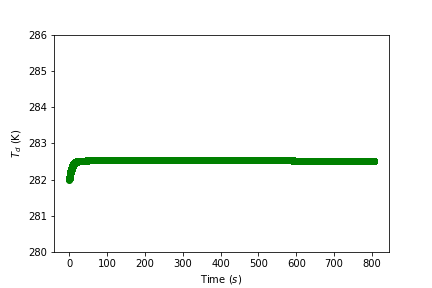
\includegraphics[width=0.8\textwidth]{heat_mass_runge_kutta_0_01_mass_lim_temp}
	\caption{$T_d$ for a droplet sized $D^2=1.1mm$ with $Re_d=0$, $T_{d_0}=282K$, $T_G=298K$, $Y_G=0$ for $\Delta t=0.01s$. Using a Runge-Kutta method.}
	\label{heat_mass_runge_kutta_0_01_mass_lim_temp}
\end{figure}

\begin{figure}[h]
	\centering
	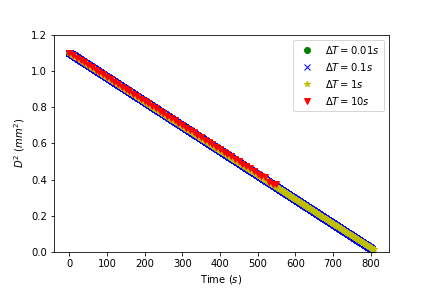
\includegraphics[width=0.8\textwidth]{heat_mass_runge_kutta_deltat_mass_lim_mass}
	\caption{$D^2$ for a droplet sized $D^2=1.1mm$ with $Re_d=0$, $T_{d_0}=282K$, $T_G=298K$, $Y_G=0$ for different $\Delta t$. Using a Runge-Kutta method.}
	\label{heat_mass_runge_kutta_deltat_mass_lim_mass}
\end{figure}

\begin{figure}[h]
	\centering
	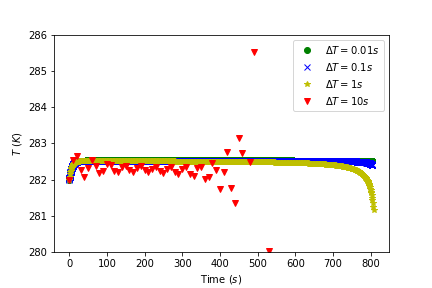
\includegraphics[width=0.8\textwidth]{heat_mass_runge_kutta_deltat_mass_lim_temp}
	\caption{$T_d$ for a droplet sized $D^2=1.1mm$ with $Re_d=0$, $T_{d_0}=282K$, $T_G=298K$, $Y_G=0$ and different $\Delta t$. Using a Runge-Kutta method.}
	\label{heat_mass_runge_kutta_deltat_mass_lim_temp}
\end{figure}
\end{document}